%% SW design: PSoC Boundary

\begin{figure}[htbp] \centering
{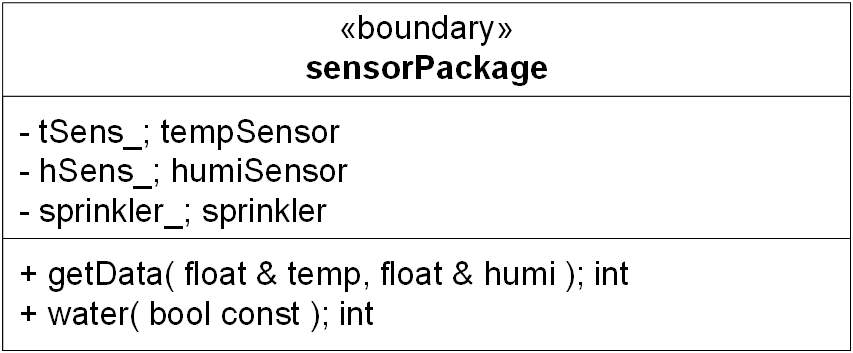
\includegraphics[scale=1.3]{filer/design/Klassediagrammer/sw_psoc_sensorPackage}}
\caption{Klasse sensorPackage}
\label{fig:sw_psoc_class_sensorPackage}
\end{figure} 

{\centering
\textbf{sensorPackage}\par
}
\textbf{Ansvar:} Holder styr på tilkoblede sensorer. \

\verb+sensorPackage( ) +\\
\textbf{Parametre:} Ingen \\
\textbf{Returværdi:} Ingen \\
\textbf{Beskrivelse:} Skal oprette sensor- og sprinklerobjekter og udføre den nødvendige opsætning af disse. \\

\verb+int getData( float * temp, float * humi )+ \\
\textbf{Parametre:} Pointers til at gemme aflæste temperatur og fugtighed i. \\
\textbf{Returværdi:} 0 ved succes ellers negativ i overenstemmelse med fejl-listen. \\
\textbf{Beskrivelse:} Aflæs data fra temperatur- og fugtighedssensor og returnere disse i de modtagende referencer. \\

\verb+int water( const unsigned char )+ \\
\textbf{Parametre:} 1 = tænd sprinkler, 0 = sluk sprinkler. \\
\textbf{Returværdi:} 0 ved succes ellers negativ i overenstemmelse med fejl-listen. \\
\textbf{Beskrivelse:} Tænd eller sluk tilkoblede sprinkler ud fra modtagende parameter. \\


\begin{figure}[htbp] \centering
{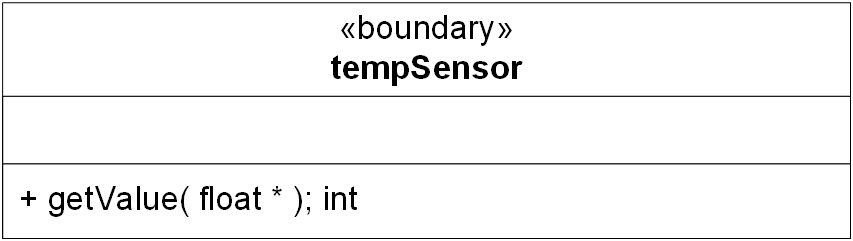
\includegraphics[scale=1.3]{filer/design/Klassediagrammer/sw_psoc_tempSensor}}
\caption{Klasse tempSensor}
\label{fig:sw_psoc_class_tempSensor}
\end{figure} 

{\centering
\textbf{tempSensor}\par
}
\textbf{Ansvar:} Håndterer kommunikationen med temperatursensor. \

\verb+tempSensor( )+ \\
\textbf{Parametre:} Ingen. \\
\textbf{Returværdi:} Ingen. \\
\textbf{Beskrivelse:} Initialiserer nødvendige indstillinger for at kunne kommunikerer med sensoren. \\

\verb+int getValue( float * )+ \\
\textbf{Parametre:} Pointer til at gemme temperatur i. \\
\textbf{Returværdi:} 0 ved succes ellers negativ i overenstemmelse med fejl-listen. \\
\textbf{Beskrivelse:} Returnerer aflæst temperatur i pointerparameteren. \\


\begin{figure}[htbp] \centering
{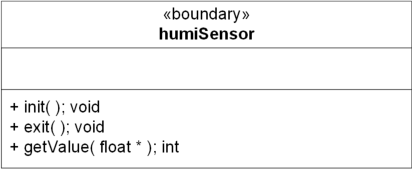
\includegraphics[scale=1.3]{filer/design/Klassediagrammer/sw_psoc_humiSensor}}
\caption{Klasse humiSensor}
\label{fig:sw_psoc_class_humiSensor}
\end{figure} 

{\centering
\textbf{humiSensor}\par
}
\textbf{Ansvar:} Håndterer kommunikationen med fugtighedssensor. \

\verb+humiSensor( )+ \\
\textbf{Parametre:} Ingen. \\
\textbf{Returværdi:} Ingen. \\
\textbf{Beskrivelse:} Initialisere nødvendige indstillinger for at kunne kommunikerer med sensoren. \\

\verb+int getValue( float * )+ \\
\textbf{Parametre:} Pointer til at gemme fugtighed i. \\
\textbf{Returværdi:} 0 ved succes ellers negativ i overenstemmelse med fejl-listen. \\
\textbf{Beskrivelse:} Returnerer aflæst fugtighed i pointerparameteren. \\

\begin{figure}[htbp] \centering
{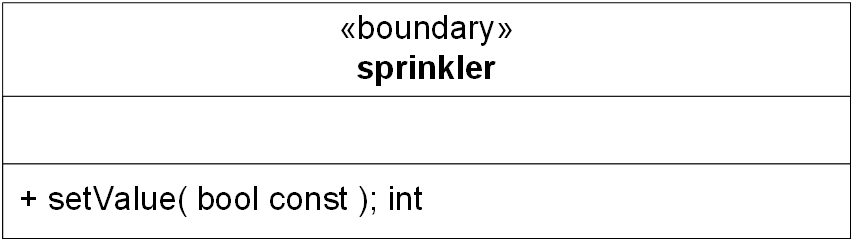
\includegraphics[scale=1.3]{filer/design/Klassediagrammer/sw_psoc_sprinkler}}
\caption{Klasse sprinkler}
\label{fig:sw_psoc_class_sprinkler}
\end{figure} 

{\centering
\textbf{sprinkler}\par
}
\textbf{Ansvar:} At aktivere og deaktivere tilkoblede sprinklere. \

\verb+sprinkler( )+ \\
\textbf{Parametre:} Ingen. \\
\textbf{Returværdi:} Ingen. \\
\textbf{Beskrivelse:} Skal initialisere nødvendige dele for at kunne bruge GPIO.\\

\verb+int setValue( unsigned char const )+ \\
\textbf{Parametre:} 1 = tænd sprinkler, 0 = sluk sprinkler. \\
\textbf{Returværdi:} 0 ved succes ellers negativ i overenstemmelse med fejl-listen. \\
\textbf{Beskrivelse:} Skal aktivere eller deaktivere sprinkler ved hjælp af GPIO.\\